软件是现代生活的重要组成部分,当软件出现错误时,开发人员需根据错误报告的描述来定位和修复错误。然而,错误报告通常由非专业人员编写,包含大量自然语言描述,这给错误定位和修复带来了很大的困难。此前,已有一篇2016年的研究调查了20世纪70年代以来与错误定位有关的大量报告\cite{7390282},该研究全面介绍了8类错误定位方法,但没有详细介绍机器学习类方法。本文将关注基于机器学习的静态错误定位方法。
\section{名词解释}
\subsection{错误定位}
错误定位方法分为静态错误定位和动态错误定位。静态错误定位仅分析源代码,不运行程序。动态错误定位需运行程序,分析程序的执行过程和测试用例的执行结果。机器学习方法主要应用于静态错误定位方法。

错误定位常用的评估指标有累积检查语句数,错误定位代价,检查得分和时间开销等。
\subsection{信息检索}
信息检索技术属于信息科学,常用于从大量的文本数据中检索出与用户需求相关的信息。基于信息检索的错误定位技术是最常见的静态错误定位方法,常被用于从错误报告中检索出与错误相关的代码片段。基于信息检索的错误定位方法主要包括以下几个步骤:
\begin{enumerate}
    \item 语料库创建:对源代码进行词法分析,去除程序关键词,分词并去除停用词,将处理后的代码片段存储在数据库中。
    \item 索引:构建单词与文件之间的索引,以便快速检索。
    \item 查询构建:处理错误报告,提取关键词,构建查询。
    \item 检索和排名:计算查询与语料库中代码片段的相似度,对代码片段进行排名。
\end{enumerate}

错误定位常用的指标大部分依赖累积检查语句数,但基于信息检索的错误定位方法必须检查所有的代码行,累积检查语句数是一个固定值,无法通过改进算法来减少。因此,通常会采用信息检索领域的评估指标,如Top K,Mean Average Precision(MAP)和Mean Reciprocal Rank(MRR)等。
\subsection{机器学习}
机器学习分为基于神经网络的方法和基于传统机器学习方法。基于神经网络的方法包括卷积神经网络(CNN),循环神经网络(RNN)等。基于传统机器学习方法包括支持向量机(SVM)和决策树等。机器学习方法的步骤如下:
\begin{enumerate}
    \item 特征提取:将源代码转换为特征向量。
    \item 数据集划分:将数据集划分为训练集和测试集。
    \item 模型训练:使用训练集训练模型。
    \item 模型评估:使用测试集评估模型。
\end{enumerate}

从2020年开始,Transformer结构的模型开始成为机器学习的主流,如BERT,GPT等。这些模型在自然语言处理领域取得了巨大的成功,也被应用于错误定位领域。

采用预训练模型的方法通常会先在大规模数据集上进行预训练,再在特定任务上进行微调。这种方法可以提高模型的泛化能力,减少过拟合的风险。其步骤与机器学习方法有一定的区别:
\begin{enumerate}
    \item 预训练:在大规模数据集上进行预训练。
    \item 微调:在特定任务上进行微调。
    \item 模型评估:使用测试集评估模型。
    \item 模型解释:解释模型的预测结果。
\end{enumerate}
\section{论文统计}
为了探索机器学习技术在静态错误定位领域的应用历史,我们通过在IEEE,ACM,Science Direct和Springer上搜索fault localization和机器学习类关键词,找到了从2013到2024的100篇论文:
\begin{figure}[H]
    \centering
    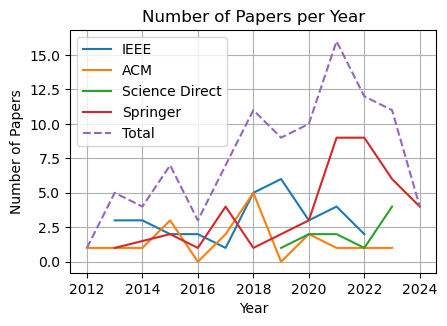
\includegraphics[width=3in]{sections/figs/articles.png}
    \caption{\label{fig1111} \xiaowuhao \hei 论文统计}
\end{figure}

可以看到,2013年静态错误定位方法开始出现,2015年达到第一个高峰,2018年达到第二个高峰,2019年开始论文增长迅速,但近两年数量有所下降。这说明,机器学习技术在错误定位领域的应用逐渐成熟,且有较大的发展空间。
